\documentclass{article}
\usepackage[utf8]{inputenc}
\usepackage[spanish]{babel}

% Necesario para usar fuentes del sistema
% \usepackage{fontspec} 
% \setmainfont{Arial} 

\usepackage{graphicx} % Required for inserting images
\usepackage{imakeidx}
\usepackage{amssymb, amsmath}
\usepackage{listings}
\usepackage{float} % Para poner las imagenes justo donde queramos

\usepackage{xcolor} % Para definir colores personalizados
\usepackage{hyperref}

\numberwithin{equation}{section} % Para las ecuaciones

% Definir un azul más oscuro
\definecolor{darkblue}{rgb}{0.0, 0.0, 1} % Azul oscuro

% Configuración personalizada para hyperref
\hypersetup{
    colorlinks=true,     % Colorear los enlaces en lugar de ponerles un recuadro
    linkcolor=blue,      % Color de los enlaces internos (por ejemplo, índice)
    citecolor=blue,      % Color de los enlaces de citas
    filecolor=magenta,   % Color de los enlaces a archivos
    urlcolor=darkblue        % Color de los enlaces a URLs
}

\makeindex
\setlength{\parindent}{12pt}


% Márgenes de página
\usepackage[left=2.5cm, right=2.5cm, top=3cm, bottom=3cm]{geometry}

% Fuente y formato
\usepackage[T1]{fontenc} % Para las ñ y letras con tilde
\usepackage{times}
\usepackage{microtype} % Mejora el espaciado de las palabras

% Encabezado y pie de página
\usepackage{fancyhdr}
\pagestyle{fancy} 
\fancyhf{}         
\rfoot{\thepage} 


\begin{document}
    \begin{titlepage}
        \centering
        {\fontsize{18pt}{22pt}\selectfont \textbf{UNIVERSIDAD ALFONSO X EL SABIO}\par}
        \vspace{1cm}
        {\fontsize{16pt}{22pt}\selectfont \textbf{ESCUELA POLITÉCNICA SUPERIOR}\par}
        \vspace{1cm}
        {\fontsize{14pt}{22pt}\selectfont \textbf{GRADO EN INGENIERÍA MATEMÁTICA}\par}
        \vspace{2cm}
        {
\includegraphics[width=1\textwidth]{img/portada.png}\par}
        \vspace{0.5cm}
        {\fontsize{20pt}{22pt}\selectfont \textbf{TRABAJO DE FIN DE GRADO}\par}
        \vspace{1cm}
        {\fontsize{14pt}{22pt}\selectfont \textbf{Computación Cuántica aplicada a la Criptografía}\par}
        \vfill
        {\fontsize{14pt}{22pt}\selectfont \textbf{Rubén Nogueras González}\par}
        \vspace{1cm}
        {\fontsize{14pt}{22pt}\selectfont \textbf{Junio de 2025}\par}
    \end{titlepage}
    
    % Pagina en blanco
    \newpage
    \thispagestyle{empty}
    \mbox{}
    \newpage

    \tableofcontents

    % Pagina en blanco
    \newpage
    \thispagestyle{empty}
    \mbox{}
    \newpage

    \listoffigures

    % Pagina en blanco
    \newpage
    \thispagestyle{empty}
    \mbox{}
    \newpage


    \section{Introducción}
        \subsection{Objetivos}

        \vspace{5mm}

        \begin{itemize}
            \item Comprender la necesidad de la mecánica cuántica en la física clásica.
            \item Entender los fundamentos matemáticos de la mecánica cuántica, incluyendo álgebra lineal y espacios de Hilbert.
            \item Aprender las diferencias, ventajas y desventajas entre un ordenador cuántico y uno tradicional.
            \item Analizar el papel que juegan las puertas cuánticas en la manipulación de estados, y por lo tanto en algoritmos cuánticos.
            \item Explicar los distintos principios básicos de la criptografía cuántica para garantizar la seguridad de los nuevos sistemas.
            \item Aprender el concepto de teleportación cuántica como mecanismo eficiente y seguro para la transmisión de información.
        \end{itemize}

        \vspace{5mm}

        \subsection{Historia de la Mecánica Cuántica}

        \vspace{5mm}

        La computación cuántica es un nuevo sistema de computación, en el que nos apoyamos en las propiedades de los sistemas cuánticos para mejorar distintos paradigmas de la computación clásica. Esto lo hacemos mediante el uso del \textit{qubit}, la unidad básica de información cuántica, a diferencia de la información clásica que se centra en el \textit{bit} como unidad minima de información. La principal ventaja de los \textit{qubits} es que, además de albergar información binaria (0 o 1), podemos obtener una mezcla de ambos estados (esto se conoce como el principio de superposición cuántica, que ya veremos en los próximos capítulos), de manera que podemos obtener algoritmos cuánticos que no pueden ser modelizados mediante \textit{bits}, reduciendo en muchos casos la complejidad de algoritmos clásicos tradicionales, lo que mejora el rendimiento y eficiencia de nuestros computadores.

        \vspace{5mm}

        Para explicar esto de la mejor manera posible, nos remontamos a los orígenes de la física cuántica, a finales del siglo \textit{XIX} y principios del siglo \textit{XX}, cuando se pensaba que la física clásica era el foco global para explicar todos los fenómenos que suceden a nuestro alrededor, hasta que con el resultado de ciertos experimentos se comenzó a ver una relación entre el comportamiento de las ondas y las partículas, rompiendo completamente con los principios de la física clásica.

        \vspace{5mm}

        En primer lugar, vamos a comenzar explicando qué es un cuerpo negro, esto es un cuerpo que absorbe toda la radiación emitida sobre él, sin reflejar nada de lo que le llega. Esto se puede imaginar como una cavidad isotérmica con un orificio por el que se aproxima cierta radiación, de manera que permanezca en su interior. Además, suponemos que dicha cavidad se encuentra en equilibrio térmico, es decir, a una temperatura constante, de manera que la radiación que permanece dentro de ella se transforma en energía, obligando a emitir radiación hacia el exterior, sin tener nada que ver con la radiación que entra por el orificio.

        \vspace{5mm}

        \begin{figure}[H]
            \centering
            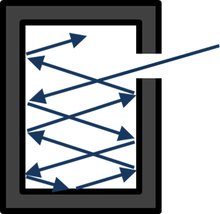
\includegraphics[width=0.2\textwidth]{img/Introduccion/cavidad_cuerpo_negro2.png}
            \caption{Ilustración del cuerpo negro}
            \label{fig: f1}
        \end{figure}
        
        \vspace{5mm}

        La física clásica es incapaz de explicar la radiación emitida por un cuerpo negro en función de la longitud de onda,
        hasta que la explicación de este fenómeno vino de la mano de \textit{Max Planck} en el siglo \textit{XX}, el cual establece que la energía liberada por el cuerpo negro se emite en pequeños paquetes, llamados \textit{cuantos de energía}. Esta energía es proporcional a una pequeña constante, la constante de Planck, de manera que la energía emitida por el cuerpo negro no es continua, sino que toma un valor discreto que ha de ser múltiplo de dicha constante por su frecuencia de onda, rompiendo completamente con la física de la época y dando el nacimiento a un nuevo campo de la física, la mecánica cuántica.

        \vspace{5mm}

        \begin{equation}
            E = h \nu
            \label{eq: planck}
        \end{equation}

        \vspace{5mm}

        Siendo \( h \) la denominada \textit{constante de Planck}, la cual alcanza un valor de \( 6.62607015 \times 10^{-34} \, \text{J} \cdot \text{s} \), y siendo \( \nu \) la frecuencia. Esta energía o intensidad que libera el cuerpo la podemos medir, en función de su longitud de onda, obteniendo la siguiente gráfica:

        \vspace{5mm}

        \begin{figure}[h]
            \centering
            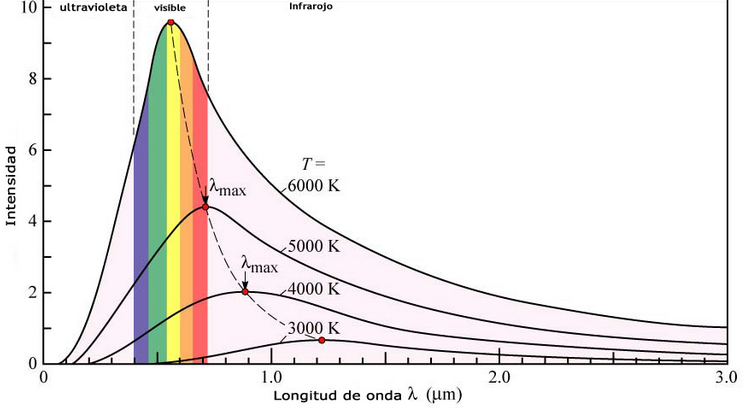
\includegraphics[width=0.75\textwidth]{img/Introduccion/catastrofe_ultravioleta.png}
            \caption{Catástrofe del ultravioleta}
            \label{fig: f2}
        \end{figure}

        \vspace{5mm}

        Podemos observar que a diferentes temperaturas (longitudes de onda) llegamos a diferentes curvas. La física clásica intentaba predecir estas curvas mediante ciertos modelos, que, aunque se ajustaban correctamente en distintas zonas de la gráfica, no se acercaban ni mucho menos a la realidad. Un ejemplo de esto es la catástrofe del ultravioleta, como resultado de no ajustarse correctamente en la zona ultravioleta, en la que la intensidad de la energía tendía a infinito como resultado de otros modelos, en lugar de tender a cero como propuso \textit{Max Planck}, formulando una ecuación que describe perfectamente la figura (\ref{fig: f2}):

        \vspace{5mm}

        \begin{equation}
            B_{\nu}(T) = \frac{2h\nu^3}{c^2} \frac{1}{e^{\frac{h\nu}{k_B T}} - 1}
            \label{eq: planck_ultravioleta}
        \end{equation}

        \vspace{5mm}

        Donde \textit{h} es la \textit{constante de Planck}, \( \nu \) la frecuencia de la radiación, \textit{c} la velocidad de la luz en el vacío, \( k_B \) la \textit{constante de Boltzmann}, \textit{T} la temperatura, y \textit{e} como base de los logaritmos naturales. No obstante, esta teoría cuántica fue primeramente descartada por los físicos de la época, al establecer que la energía no es un valor continuo sino discreto, hasta que con la llegada del efecto fotoeléctrico de \textit{Albert Einstein} todo comenzó a cobrar sentido.

        \vspace{5mm}    

        A finales del siglo XIX, en 1888, se presenta el efecto fotoeléctrico, definido por \textit{Heinrich Hertz}, que consiste en la emision de electrones (fotoelectrones) al incidir luz sobre un metal, actuando como cátodo, los cuales se recogen en un ánodo, generando corriente en un circuito. Dicha luz suele ser ultravioleta, aunque en algunos casos puede ser visible.

        \vspace{5mm}

        Previamente al experimento, se plantearon varias hipótesis en base a la física clásica de la época:

        \begin{itemize}
            \item El aumento de la intensidad de la luz incrementaría la energía cinética de los fotoelectrones emitidos.
            \item A mayor frecuencia mayor intensidad de corriente en el circuito. 
        \end{itemize}

        \vspace{5mm}

        Los resultados de dicho experimento fueron sorprendentes, ya que se observó que la energía cinetica de los electrones que poseen el cátodo no dependen de la intensidad de la luz, sino de su frecuencia, y adicionalmente se pudo ver que a mayor intensidad de luz mayor intensidad de corriente. Más tarde, en 1905, se presentó un artículo, ciertamente atrevido teniendo en cuenta los recursos de la época, que resolvía todos estos problemas.

        \vspace{5mm}

        \textit{Albert Einstein} presentó su hipótesis para el efecto fotoeléctrico, basándose en los resultados del experimento de \textit{Planck}, aclarando que la luz no se comporta como una onda, sino que está compuesta de pequeñas partículas, llamadas \textit{fotones}, cuya energía depende de su frecuencia, como ya propuso \textit{Max Planck} en (\ref{eq: planck}), rompiendo de nuevo con los principios de la física clásica.

        \vspace{5mm}

        En dicha hipótesis se establece la necesidad de una frecuencia mínima, denominada frecuencia umbral, para que el efecto fotoeléctrico tenga lugar, la cual depende del material del que esté construido el cátodo. Por lo que si la frecuencia de los \textit{fotones} emitidos por el haz de luz es menor a esta frecuencia umbral, no se produce corriente en el circuito, por muy intensa que sea la luz. De esta manera, si la frecuencia es mayor o igual a la umbral, los \textit{fotoelectrones} se trasladarán hacia el ánodo al ser expulsados del núcleo de sus átomos, generando energía cinética y por lo tanto, intensidad de corriente en el circuito. Esto lo podemos razonar con la siguiente ecuación:

        \vspace{5mm}

        \begin{equation}
            E_e = E_{ionizacion} + E_{cinetica}
            \label{eq: einstein_fotoelectrico}
        \end{equation}

        \vspace{5mm}

        Esta ecuación tiene sentido visto lo anterior, de manera que la energía de los electrones del cátodo ha de ser igual a su \textit{energía de ionización} (o también conocido como \textit{trabajo de extracción}), la cual es la cantidad de energía necesaria para que se produzca el efecto fotoeléctrico, sumado a su \textit{energía cinética}. Por la explicación vista anteriormente, sabemos que dicha \textit{energía de ionización} depende de la \textit{frecuencia umbral \( \nu_{0} \)}, y con la ecuación de la energía de \textit{Planck} (\ref{eq: planck}), además de conocer la \textit{energía cinética} de una partícula, podemos desarrollar la expresión (\ref{eq: einstein_fotoelectrico}):

        \vspace{5mm}

        \begin{equation*}
            h \nu = h \nu_{0} + \frac{1}{2} m_{e} v_{e}^{2}
        \end{equation*}

        \vspace{5mm}

        Donde \textit{h} es la \textit{constante de Planck}, \( \nu \) es la \textit{frecuencia}, \( \nu_{0} \) es la \textit{frecuencia umbral}, \( m_{e} \) es la masa del electrón, y \( v_{e} \) la velocidad del electrón, en este caso al cuadrado. 
        
        \vspace{5mm}

        Estos son solo dos de los múltiples experimentos con soluciones extrañas para los físicos clásicos de aquella época, en los que, como hemos visto, el comportamiento de ciertos fenómenos, teóricamente imaginados como funciones de onda, se comportan como partículas. También se da el fenómeno contrario, experimentos planteados como partículas pero que son razonados mediante funciones de onda. Esto se definió con el nombre de \textit{dualidad onda-corpúsculo}.
        
        \vspace{5mm}

        Más tarde, tras estudiar a fondo las bases de la mecánica cuántica propuesta por \textit{Max Planck} y \textit{Albert Einstein}, \textit{Louis de Broglie} propuso en su tesis doctoral, en \textit{1924}, que no solo la luz tiene un carácter ondulatorio, sino que toda partícula material, como los electrones, tienen una naturaleza ondulatoria, cuya longitud de onda \( \lambda \) es:
        
        \vspace{5mm}

        \begin{equation}
            \lambda = \frac{h}{p}
            \label{eq: longitud de onda}
        \end{equation}

        \vspace{5mm}

        Donde \textit{p} se refiere al \textit{momento lineal} de la partícula, lo cual podemos expresar como \( p = m \cdot v \), siendo \textit{m} la masa, y \textit{v} la velocidad de la partícula. Tras el razonamiento de \textit{Broglie} en \textit{1924}, surge la \textit{función de onda} en una dimensión, la cual describe el comportamiento las partículas con carácter ondulatorio:

        \vspace{5mm}

        \begin{equation}
            \varphi (x, t) = e^{i(px - Et) / \hbar}
            \label{eq: funcion_de_onda}
        \end{equation}

        \vspace{5mm}

        Siendo \textit{i} la unidad imaginaria, \( \hbar \) la \textit{constante de Planck normalizada}

        \vspace{5mm}

        \begin{equation}
            \hbar = \frac{h}{2\pi} 
            \label{constante_planck_normalizada}
        \end{equation}    

        \vspace{5mm}
        
        y \textit{x} y \textit{t} las coordenadas de posición y tiempo de la partícula. Sin embargo, todavia no se conocia su significado fisico con total exactitud. No fue hasta que con el experimento de la doble rendija de \textit{Clinton Davisson} y \textit{Lester Germer} sobre electrones en \textit{1927} (aunque \textit{Thomas Young} lo propuso en \textit{1801}, sobre un haz de luz, demostrando su naturaleza ondulatoria) que se confirmó la hipótesis de \textit{De Broglie}. Como su propio nombre indica, dicho experimento consiste en una superficie opaca con dos rendijas, detrás de la cual colocamos un detector de partículas para poder percibir el comportamiento de los electrones o fotones que pasan a través de ambas rendijas. Según la física clásica, se espera que las partículas pasen a través de las rendijas en forma de línea recta, como lo haría cualquier objeto. Sin embargo, esto no sucede así en el contexto de la mecánica cuántica.

        \vspace{5mm}

        \begin{figure}[h]
            \centering
            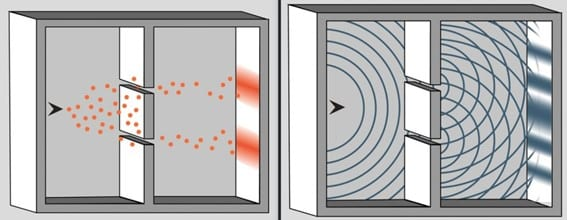
\includegraphics[width=0.75\textwidth]{img/Introduccion/doble_rendija.png}
            \caption{Experimento de la doble rendija}
            \label{fig: doble_rendija}
        \end{figure}

        \vspace{5mm}

        Al realizar el experimento, podemos observar un patrón de interferencias en la pantalla de detección situada detrás de las rendijas, el cual es muy similar al patrón que siguen las ondas cuando se superponen unas con otras. Efectivamente, las ondas asociadas a cada partícula se superponen unas con otras como se reveló en el experimento, no obstante, cuando observamos estas partículas mediante el detector, se comportan como una partícula clásica, cambiando su comportamiento, de manera que podemos ver por qué rendija cruzó la partícula. Este fenómeno se conoce como \textit{colapso de función de onda}, y existen muchas teorías que intentar explicar esto, siendo la más famosa la \textit{intepretación de Copenhage}, en la que se establece que la observación de la partícula produce un colapso de su función de onda, determinando su estado correspondiente a la medición.

        \vspace{5mm}

        Matemáticamente, podemos expresar la superposición de ondas como una superposición de estados, esto es:

        \vspace{5mm}

        \begin{equation}
            \psi(x, t) = \psi_{1}(x, t) + \psi_{2}(x, t) + \dots + \psi_{n}(x, t), \qquad \forall n \in \mathbb{N} \setminus \{0\}
            \label{eq: superposicion}
        \end{equation}

        \vspace{5mm}

        Adicionalmente, surgieron ciertas dudas relacionadas con la naturaleza de la función de onda. Es lógico preguntarse que, si las partículas están definidas por funciones de onda, ¿Dónde están realmente las partículas? Ya que una partícula no puede estar en varios puntos a la vez, ha de estar en un único punto. Es aquí cuando entró \textit{Max Born}, quien sugiere que \( \lvert \psi(x, t) \rvert ^ {2} \) no es simplemente el cuadrado del módulo de la función de onda, sino que es una función de densidad de probabilidad, de manera que, para cada instante de tiempo y una región del espacio, la siguiente integral

        \vspace{5mm}

        \begin{equation}
            \int_{E} \lvert \psi(x, t) \rvert ^ {2} dx, \qquad \forall t \in \mathbb{R}, E \subset \Omega
            \label{eq: densidad_probabilidad_onda}
        \end{equation}

        \vspace{5mm}

        Representa la densidad de probabilidad de encontrar una partícula para un valor de \textit{t} en una determinada región \textit{E} del espacio \( \Omega \), de manera que podemos deducir una condición que ha de cumplir la expresión (\ref{eq: densidad_probabilidad_onda}):
        
        \vspace{5mm}

        \begin{equation}
            \int_{\Omega} \lvert \psi(x, t) \rvert ^ {2} dx = 1, \qquad \forall t \in \mathbb{R}
        \end{equation}

        \vspace{5mm}
        
        Esto tuvo una importancia bastante profunda en la mecánica cuántica de la época y en la física en general, ya que las únicas ideas de probabilidad estaban relacionadas a sistemas de incertidumbre, como el lanzamiento de una moneda. De esta manera se concluyó en la probabilidad como uno de los principales focos de la física y de la comprensión de las partículas subatómicas.

        \vspace{5mm}

        Esto concluye, al no poder medir con exactitud el estado de una partícula, como ocurre en la física clásica, en el \textit{principio de incertidumbre} de \textit{Heisenberg} en \textit{1927}, estableciéndose que en la medición de una partícula no podemos conocer con completa exactitud la posición y el momento lineal a la vez, sino que cuanto más preciso midamos su posición exacta menos precisa será la medición del momento lineal de dicha partícula y viceversa.

    \vspace{5mm}

    \section{Ecuación de Schrödinguer}

    \subsection{Obtención de la Ecuación de Schrödinguer}

    \vspace{5mm}

    Todas las ideas vistas anteriormente, la función de onda (\ref{eq: funcion_de_onda}), la superposición cuántica (\ref{eq: superposicion}) y la interpretacion probabilística de la función de onda (\ref{eq: densidad_probabilidad_onda}) dieron lugar a la necesidad de decribir la evolución de la función de onda \( \psi(x, t) \) en función del tiempo \textit{t}. Es en este momento cuando aparece \textit{Erwin Schrödinguer} en \textit{1926}, presentando su famosa ecuación, obtenida de derivar y desarrollar la ecuación  (\ref{eq: funcion_de_onda}). 
    
    En primer lugar, derivamos (\ref{eq: funcion_de_onda}) con respecto al tiempo \textit{t}:
    \begin{align*}
        \frac{\partial}{\partial t} \psi(x, t) &= \frac{\partial}{\partial t} e^{i(px - Et) / \hbar} \\[8pt]
        \frac{\partial}{\partial t} \psi(x, t) &= e^{i(px - Et) / \hbar} \left(- \frac{iE}{\hbar} \right)
    \end{align*}
    Podemos observar que vuelve a aparecer la función de onda (\ref{eq: funcion_de_onda}), al tratarse de una función exponencial:
    \begin{equation*}
        \frac{\partial}{\partial t} \psi(x, t) = - \frac{iE}{\hbar} \psi(x, t)
    \end{equation*}
    A continuación multiplicamos ambos miembros por \( i\hbar \), para eliminar los denominadores y substrayendos de la expresión:
    \begin{equation}
        i \hbar \frac{\partial}{\partial t} \psi(x, t) = E \psi(x, t)
        \label{eq: obtencion_schrodinguer}
    \end{equation}
    Esta expresión la reservaremos para más adelante, ya que, en los siguientes cálculos, necesitaremos el producto de la energía del sistema \( E \) y la función de onda \( \psi \). Como siguiente paso, vamos a continuar derivando la función de onda (\ref{eq: funcion_de_onda}) con respecto de \textit{x}:
    \begin{align*}
        \frac{\partial}{\partial x} \psi(x, t) &= \frac{\partial}{\partial x} e^{i(px - Et) / \hbar} \\[10pt]
        \frac{\partial}{\partial x} \psi(x, t) &= e^{i(px - Et) / \hbar} \left( \frac{ip}{\hbar} \right) \\[10pt]
        \frac{\partial}{\partial x} \psi(x, t) &= \frac{ip}{\hbar} \psi(x, t)
    \end{align*}
    Derivamos por segunda vez respecto de la variable espacial:
    \begin{align*}
        \frac{\partial}{\partial x^{2}} \psi(x, t) &= \frac{\partial}{\partial x} \left( \frac{ip}{\hbar} \psi(x, t) \right) \\[10pt]
        \frac{\partial}{\partial x^{2}} \psi(x, t) &= - \frac{p^{2}}{\hbar^{2}} \psi(x, t)
    \end{align*}
    Multiplicamos por (\( - \frac{\hbar^{2}}{2m} \)) para obtener lo siguiente:
    \begin{equation*}
        - \frac{\hbar^{2}}{2m} \frac{\partial}{\partial x^{2}} \psi(x, t) = \frac{p^{2}}{2m} \psi(x, t)
        \\[2mm]
    \end{equation*}
    Conociéndose que la energía cinética es \( E = \frac{p^{2}}{2m} \), obtenemos la siguiente expresión
    \begin{equation*}
        - \frac{\hbar^{2}}{2m} \frac{\partial}{\partial x^{2}} \psi(x, t) = E \psi(x, t)
    \end{equation*}
    Sustituyendo el valor que acabamos de obtener \( E \psi(x, t) \) en (\ref{eq: obtencion_schrodinguer}), llegamos prácticamente a la ecuación que estamos buscando:
    \begin{equation*}
        i \hbar \frac{\partial}{\partial t} \psi(x, t) = - \frac{\hbar^{2}}{2m} \frac{\partial}{\partial x^{2}} \psi(x, t)
        \\[2mm]
    \end{equation*}
    Para terminar, si agregamos la energía potencial y generalizamos la ecuación para más de una dimensión espacial, obtenemos la famosa \textbf{\textit{ecuación de Schrödinguer}}:
    \begin{equation}
        \boxed{i \hbar \frac{\partial}{\partial t} \psi(x, t) = (- \frac{\hbar^{2}}{2m} \Delta + V(x, t)) \psi(x, t)} 
        \label{eq: ecuacion_schrodinguer}     
    \end{equation}
    Siendo \( \Delta \) el operador Laplaciano en coordenadas canónicas, que se define como
    \begin{equation*}
        \Delta = \frac{\partial}{\partial^{2} x_{1}} + \cdots + \frac{\partial}{\partial^{2} x_{n}}, \qquad \forall n \in \mathbb{N}
    \end{equation*}

    \vspace{5mm}

    \subsection{La Ecuación de Schrödinguer Independiente del Tiempo}

    \vspace{5mm}

    A continuación, para obtener la \textit{ecuación de Schrödinguer independiente del tiempo} tenemos que plantearnos obtener las soluciones de la ecuación de Schrödinguer (\ref{eq: ecuacion_schrodinguer}). Para simplificar cálculos, vamos a suponer que la energía potencial \( V(x) \) en (\ref{eq: ecuacion_schrodinguer}) depende única y exclusivamente de la variable espacial \textit{x}, de manera que podemos probar a encontrar soluciones por el método de \textit{separación de variables}. Supongamos una solución como producto de dos funciones \( \psi(x) \) y \( \tau(t) \):

    \begin{equation*}
        \Psi(x, t) = \psi(x) \tau(t) \\[5pt]
    \end{equation*}

    Sustituyendo en (\ref{eq: ecuacion_schrodinguer}) nos queda como

    \begin{equation*}
        i \hbar \frac{\partial}{\partial t} \psi(x) \tau(t) = \left( - \frac{\hbar^{2}}{2m} \Delta + V(x) \right) \psi(x) \tau(t) \\[5pt]
    \end{equation*}

    Podemos dividir entre \( \psi(x) \tau(t) \) y ordenar ambos miembros, de manera que un miembro nos quede únicamente en función de \textit{x} y otro en función de \textit{t}:

    \begin{equation*}
        i \hbar \frac{1}{\tau(t)} \frac{\partial}{\partial t} \tau(t) = V(x) - \frac{\hbar^{2}}{2m} \frac{1}{\psi(x)} \frac{\partial}{\partial x^{2}} \psi(x) \\[5pt]
    \end{equation*}

    Hemos de recalcar que hemos tomado el laplaciano \( \Delta \) como \( \frac{\partial}{\partial x^{2}} \), siendo este el laplaciano en una dimensión espacial, con el fin de simplificar los cálculos. Llegados a este punto, para que se cumpla la igualdad, cada miembro de la ecuación ha de ser igual a una constante \( E \), al demostrarse que se trata de una ecuación separable
    
    \begin{equation}
        \begin{cases}
            \displaystyle i \hbar \frac{1}{\tau(t)} \frac{\partial}{\partial t} \tau(t) = E \\[10pt]
            \displaystyle V(x) - \frac{\hbar^{2}}{2m} \frac{1}{\psi(x)} \frac{\partial}{\partial x^{2}} \psi(x) = E \\[10pt]
        \end{cases}
        \label{eq: separacion_variables}
    \end{equation}

    Tomando como base la primera ecuación del sistema, podemos obtener una solución exponencial de la siguiente manera:
        
    \begin{align*}
        \frac{\partial}{\partial t} \tau(t) &= \frac{E}{i \hbar} \tau(t) \\[10pt]
        \tau(t) &= e ^ { \left( - \frac{Ei}{\hbar} \right) t}
    \end{align*}

    Esto nos proporciona una evolución temporal del sistema en el que se encuentra la partícula. Sin embargo, para obtener la ecuación que estamos buscando, hemos de fijarnos en la segunda ecuación de (\ref{eq: separacion_variables}):

    \begin{equation*}
        V(x) - \frac{\hbar^{2}}{2m} \frac{1}{\psi(x)} \frac{\partial}{\partial x^{2}} \psi(x) = E
    \end{equation*}

    La cual podemos reescribir como

    \begin{equation}
        \left( - \frac{\hbar^{2}}{2m} \frac{\partial}{\partial x^{2}} + V(x) \right) \psi(x) = E \psi(x) \\[5pt]
        \label{eq: schrodinguer_independiente_tiempo}
    \end{equation}

    En muchas referencias, la ecuación (\ref{eq: schrodinguer_independiente_tiempo}) es ya la ecuación que estamos buscando. Sin embargo, nosotros la vamos a denotar en función del operador \textit{Hamiltoniano} \( H \), el cual representa la energía total de nuestro sistema cuando ésta permanece constante en el tiempo, que en nuestro caso sucede al establecer que \( V(x, t) = V(x) \). Así, la \textbf{\textit{ecuación de Schrödinguer independiente del tiempo}} queda como
    
    \begin{equation}
        \boxed{ H \psi(x) = E \psi(x)}
        \label{eq: schrodinguer_independiente_tiempo_hamiltoniano}
    \end{equation}

    Siendo \( H = \left( - \frac{\hbar^{2}}{2m} \frac{\partial}{\partial x^{2}} + V(x) \right) \) el operador \texit{Hamiltoniano}. Finalmente, podemos concluir que la solución completa queda como

    \begin{equation}
        \Psi(x, t) = e ^ { \left( - \frac{Ei}{\hbar} \right) t} \psi(x)
    \end{equation}

    \vspace{5mm}

    La ecuación (\ref{eq: schrodinguer_independiente_tiempo_hamiltoniano}) describe los estados estacionarios de una partícula en el potencial \( V(x) \) y es usada en muchos sistemas físicos de vital importancia (generalmente aquellos cuyo potencial no depende del tiempo \( t \)) como átomos y moléculas en estado estacionario, siempre y cuando el sistema se encuentre en equilibrio y no haya fuerzas externas que varíen el valor de la energía potencial con respecto al tiempo, pozos de potencial infinito, osciladores armónicos, o campos eléctricos y gravitacionales constantes.

    \vspace{5mm}

    Sin embargo, hay otras muchas situaciones en las que el potencial no solo depende de la posición \( x \), de manera que no podemos aplicar el método de separación de variables visto anteriormente, como partículas en campos magnéticos, problemas asociados a la relatividad, o sistemas caóticos. Para estos sistemas utilizamos otros métodos de resolución, como simulaciones numéricas, para alcanzar la solución del sistema.

    \vspace{5mm}

    \subsection{El Espacio de Hilbert}
    \section{Álgebra Lineal y Puertas Cuánticas}
    \subsection{Estados Cuánticos}
    \subsubsection{Esfera de Bloch}    
    \subsection{Producto Escalar}
    \subsubsection{Ortonormalidad}
    \subsection{Puertas Cuánticas}
    \subsection{Producto Tensorial}
    \section{Errores Cuánticos}
    \subsection{Decoherencia}
    \subsection{Shor Code}
    \section{Entrelazamiento Cuántico}
    \subsection{Estados de Bell}
    \subsection{Codificación Superdensa}
    \section{Teleportación Cuántica}
    \section{Algoritmos Cuánticos}
    \subsection{Oracles Cuánticos}
    \subsection{Algoritmo de Grover}
    \subsection{Algoritmo de Shor}

    \section{Estado del Arte}

    \vspace{5mm}

    La empresa líder en computación cuántica es, hasta la fecha y sin duda alguna, IBM, la cual ofrece a nuestra disposición distintas páginas web en las que podemos ejecutar circuitos cuánticos y ver su comportamiento de la manera más real posible. El desarrollo del circuito se hace a través de \textit{Python} mediante su librería destinada a la computación cuántica \textit{Qiskit}, y una vez lo hemos completado, tenemos distintas opciones de configuración para la ejecución del circuito.

    \vspace{5mm}

    Por otra parte, si la programación en \textit{Python} no es nuestro punto fuerte, tenemos a nuestra disposición la interfaz gráfica para el desarrollo de circuitos cuánticos de IBM, Quantum Composer. Con esta herramiento web podemos crear circuitos cuánticos con el sistema \textit{drag and drop} sobre puertas cuánticas o qubits, de manera que se genera el correspondiente código equivalente al circuito cuántico creado y se ejecuta en un emulador o sistema cuántico, además de que podemos visualizar el estado y la fase correspondiente en la \textit{esfera de Bloch}, y un histograma con las probabilidades de los estados a los que puede colapsar el circuito.
    
    \vspace{5mm}

    De la misma manera que IBM, Amazon ha desarrollado su propia plataforma para la ejecución de circuitos cuánticos, la cual está basada nuevamente en \textit{Python}, con la diferencia de que usamos la librería relacionada con su propio producto, \textit{Braket}. Este producto incluye ciertas ventajas sobre el producto de IBM, como que permite la combinación de computación cuántica y clásica, aunque como vimos anteriormente, todo circuito clásico se puede expresar como un circuito cuántico. Tambień podemos encontrar productos de otras empresas para la simulación y ejecución de circuitos cuánticos, como Google o Azure, pero no dejan de ser, junto con el producto de Amazon, competidores de la solución presentada por IBM, la cual fue la primera en salir públicamente al mercado con su plataforma IBM Quantum Experience, lanzada en \textit{2016}.

    \vspace{5mm}

    No obstante, la computación cuántica tiene muchos problemas, relacionados precisamente con la naturaleza de las partículas subatómicas, las cuales son muy sensibles al ruido causado por el exterior, lo que hace que se produzcan muchos fallos en los circuitos y que, por lo tanto, los computadores cuánticos actuales no sean tolerantes a fallos (\textit{fault-tolerant}), de manera que los errores se acumulan muy rápidamente y sin la capacidad de ser revertidos con la tecnología cuántica hasta el momento. Sin embargo, Microsoft ha hecho un hallazgo que puede convertirse en la revolución del siglo, mucho más allá que el desarrollo de la inteligencia artificial en estos últimos años.

    \vspace{5mm}

    Microsoft ha anunciado el lanzamiento de \textit{Majorana 1}, la primera unidad de procesamiento cuántico (QPU) con qubits topológicos, qubits que almacenan informacion cuántica de manera más estable y robusta, de manera que es mucho menos susceptible a errores cuánticos, que es uno de los principales problemas de este campo de la física y la tecnología, siendo una de las principales motivaciones para Microsoft construir el primer ordenador cuántico con tolerancia a fallos en los próximos años.

    \vspace{5mm}

    La clave de este gran avance ha sido el desarrollo de materiales topoconductores, los cuales permiten la superconductividad topológica, un estado de la materia que hasta este descubrimiento solo existía en la teoría. Este tipo de materiales se crean con arseniuro de indio y aluminio, de manera que cuando se enfrían prácticamente al cero aboluto y se sintonizan con campos magnéticos, se forman nanocables superconductores topológicos con modos cero de Majorana (MZM) en sus extremos, de manera que aumentan la estabilidad y se reducen los errores en comparación con los qubits tradicionales.
    \vspace{5mm}

    Así es como se ha desarrollado el primer qubit topológico del mundo, y se plantea tener un chip cuántico con más de un millón de qubits y tolerante a fallos en unos años, y no en unas décadas como se planteaba anteriormente, dando un gran paso en la computación cuántica práctica y probablemente uno de los mayores hitos de este campo.

    % Pagina en blanco
    \newpage
    \thispagestyle{empty}
    \mbox{}
    \newpage

    \section{Bibliografía}

        \vspace{5mm}

        TFG Silvia Rodriguez\par
        \url{https://matematicas.uam.es/~fernando.chamizo/supervision/TFG/past/memoirs/TFG\_silvia\_rodriguez.pdf}
        \vspace{2mm}

        Investigacion Computacion Cuantica --> Seguridad informatica, redes informaticas, IA, etc.\par
        \url{https://rua.ua.es/dspace/bitstream/10045/124691/1/Estudio\_de\_la\_computacion\_cuantica\_en\_los\_diferent\_Claramunt\_Carriles\_Sergio.pdf}
        \vspace{2mm}

        Universidad de Murcia --> Schrodinguer, Hamiltoniano, Oscilador armonico, Atomo de Hidrogeno\par
        \url{https://webs.um.es/gustavo.garrigos/tfg/MarinMunoz\_Diego\_TFG\_julio2021.pdf}
        \vspace{2mm}

        TFG Pablo --> Algoritmo de Grover y otros algoritmos\par
        \url{https://rodin.uca.es/bitstream/handle/10498/27218/tfg\_pablo.pdf?sequence=1\&isAllowed=y}
        \vspace{2mm}

        TFM --> Schrodinguer e interpretacion probabilistica de la funcion de onda\par
        \url{https://repositorioinstitucional.buap.mx/server/api/core/bitstreams/fb9bfe95-7945-404d-a3c5-00ba77b8ad71/content}
        \vspace{2mm}

        Universidad Autonoma de Madrid --> Interpretacion probabilistica de la funcion de onda e introduccion al atomo de hidrogeno\par
        \url{https://matematicas.uam.es/~fernando.chamizo/supervision/TFG/past/memoirs/TFG\_luis\_sanchez.pdf}
        \vspace{2mm}

        TFG --> Espacios de Hilbert y su relacion con la mecanica cuantica\par
        \url{https://idus.us.es/server/api/core/bitstreams/4c49766a-cdfc-4d72-9acf-f62761db63fb/content}
        \vspace{2mm}

        Claudia Mielgo --> El sistema cuantico es un espacio de Hilbert, y funciones de onda\par
        \url{https://matematicas.uam.es/~fernando.chamizo/supervision/TFG/past/memoirs/TFG\_claudia\_mielgo.pdf}
        \vspace{2mm}

        Algebra Lineal --> Algebra lineal, espacios de Hilbert y criptografia cuantica\par
        \url{https://repositorio.ual.es/bitstream/handle/10835/9810/VILLASANA%20ALCARAZ%2C%20MARIA%20DEL%20MAR.pdf}
        \vspace{2mm}

        Roberto Gonzalez --> Sistema Bineario e introduccion a los qubits\par
        \url{https://oa.upm.es/69234/1/TFG\_ROBERTO\_GONZALEZ\_RIVAS.pdf}
        \vspace{2mm}

        Por que un ordenador cuantico?\par
        \url{https://zaguan.unizar.es/record/76803/files/TAZ-TFG-2018-3072.pdf}
        \vspace{2mm}

        Radiacion del cuerpo negro\par
        \url{https://www.fisicacuantica.es/la-radiacion-del-cuerpo-negro/}
        \vspace{2mm}

        \url{https://weblab.deusto.es/olarex/cd/kaernten/BBR_ES_new_27.09.2013/distribucin_de_la_energa.html}
        \vspace{2mm}

        \url{https://www.quimicafisica.com/teoria-cuantica/la-radiacion-del-cuerpo-negro.html}
        \vspace{2mm}

        Efecto Fotoeléctrico\par
        \url{https://es.khanacademy.org/science/ap-chemistry/electronic-structure-of-atoms-ap/bohr-model-hydrogen-ap/a/photoelectric-effect}
        \vspace{2mm}

        \url{https://www.quimicafisica.com/teoria-cuantica/el-efecto-fotoelectrico.html}
        \vspace{2mm}

        Experimento de la Doble Rendija\par
        \url{https://www.fisicalab.com/apartado/cantidad-movimiento#google_vignette}
        \vspace{2mm}

        \url{https://www.dciencia.es/fisica-cuantica-el-experimento-de-la-doble-rendija/}
        \vspace{2mm}

        \url{https://mecanicosvalencia.es/max-born-mecanica-cuantica/}
        \vspace{2mm}

        Majorana\par
        \url{https://news.microsoft.com/source/latam/noticias-de-microsoft/microsoft-presenta-majorana-1-el-primer-procesador-cuantico-del-mundo-impulsado-por-qubits-topologicos/}
        \vspace{2mm}
    
\end{document}